\chapter{自动化的流体仿真框架}
\label{sec:sig23}

% Sec 4.1
\section{背景与动机}
我们已经描述了应用于CG上的LBM方法,但是对于工业应用来说,以上的方法完全无法满足。在工业领域中,更多注重XXXXXX,风洞测试用的更多。在这一章中我们将介绍一个基于LBM的虚拟风洞测试系统,以克服这一问题。第~\ref{sec:siga21} 章所描述的混合方法虽然高效,但不适合虚拟风洞的应用,因为此时边界层已经非常薄,远小于网格大小,从而在网格层面假设速度是线性的已经不够精确。

\paragraph{风洞与虚拟风洞}
虽然汽车行业在早期,并不注重空气动力学的影响,许多汽车的造型都以方正和硬朗为特点,但随着汽车越来越注重经济性,尤其是现在进入电动汽车的时代后,空气动力学对汽车造型的设计影响越来越显著。从20世纪早期开始,航空工程师开始使用风洞来测试飞机,之后汽车的设计制造也开始使用类似的技术。随后更多的领域开始使用风洞测试进行空气动力学特性的测试,如高层建筑物、高速列车、船舰等的设计。虽然风洞实验对产品设计有着很强的指导意义,但是真实的风洞实验需要进行实际的物理建模,并且风洞本身的造价也十分高昂。这样的高成本与操作难度,使其难以被频繁应用。在计算机得以发展后,虚拟风洞随即出现,并成为一种更简单、高效、节约成本的气动设计解决方案。同时虚拟风洞可以更直观地提供可视化结果,如表面的高压与低压区分布、不同位置的气流的涡流程度等。这些数据可以在设计的迭代中节约大量的时间与经济成本。直到今天,虚拟风洞的效率依然深刻影响汽车、建筑、航空航天等领域的产品研发周期~\cite{HighriseBuildings,windScience}。

\paragraph{虚拟风洞的现状}
对于最常见的亚声速弱可压情况 (马赫数小于0.3时,此时流体依然可以用不可压模型进行近似描述),目前的虚拟风洞测试需要经过一个非常耗时的前处理阶段。最耗时的部分是基于物体模型构建贴体的计算网格,这一过程需要大量的人工调整,以保证网格质量。构建好计算网格后,使用基于有限体积或有限元的CFD求解器,来求解流体。即使在CPU集群上,进行这样的流体求解也可能需要数天才可完成一次仿真。在GPU平台上,使用现有软件,如西门子StarCCM+~\cite{Siemens},进行瞬态流求解,也是类似的效率。所以更多时候,在现有的虚拟风洞实验中会进行稳态求解,以节省计算时间。

\paragraph{使用LBM进行气动分析}
近些年来,LBM在进行高效湍流仿真上,已经取得了长足的进步。LBM在核心算法上的进展已经使其有能力在大规模并行结构上高效求解流体,并达到满足工业应用的精度范围~\cite{Li-2020,Lallemand:2021}。这使得LBM开始在CFD领域成为传统方法之外的一个新的选项 (我们注意到现有的工业软件,如PowerFLOW与XFlow~\cite{Simulia}均基于LBM开发,但其具体使用的方法模型并不明确)。在CG领域,虽然有LBM方法得到了较好的视觉结果~\cite{Li-2020,Lyu:2021},但其精度依然远比不上工业应用所需的精度。

\paragraph{我们的工作}
我们尝试通过解决一些LBM中的关键问题,提升LBM的整体能力,使得LBM可以成为一个统一的流体仿真框架,以应用到视觉特效、工业设计等多个领域。通过提升碰撞模型、边界处理的精度,结合多分辨率网格与GPU优化,我们构建了一个虚拟的亚声速弱可压风洞测试系统。该系统可以拥有与现有的CFD商业软件相似、甚至更高的精度与计算效率。

% Sec 4.2
\section{方法}
我们的系统相比于现有的LBM主要包含以下四个方面的改进:
\begin{itemize}
	\item 我们对累积量碰撞模型,通过局部熵值的最大化的原则进行了改进。改进后的碰撞模型在精度上有所提升,并可在$10^8$级别的雷诺数下保持稳定; 
	\item 我们提出了一个新的单点插值反弹边界来处理静态与动态物体边界,可以更精准地求解边界层流场;
	\item 我们提出了一个多分辨率网格构建算法,以自动且灵活地构建多分辨率网格,可以在不需花费过多人工前处理的情况下,完成高分辨率流体仿真
	\item 我们还提出了一系列的GPU优化,进一步提升运算效率。
\end{itemize}

我们将在下面依次介绍这四部分内容。

\subsection{累积量碰撞模型的高阶参数优化}
在碰撞过程中,高阶松弛系数对仿真 (尤其是湍流仿真) 有着很大的影响。Li等~(\citeyear{Li-2020}) 讨论了在中心矩碰撞方法中,进行高阶参数优化的方法。作者通过回归方法,自适应地调整参数,降低了数值色散和耗散误差,提高了数值精度。于是我们希望同样将高阶松弛系数的优化引入累积量碰撞模型中。由于累积量模型的空间变换是非线性的,我们无法直接应用Li等~(\citeyear{Li-2020}) 中的回归方法,或Kramer等~(\citeyear{Kramer-2019}) 中的熵优化方法。但是,我们可以通过一定的推导,将Kramer等~(\citeyear{Kramer-2019}) 中的熵优化方法推广至累积量碰撞模型中。下面我们介绍推导过程。

首先,我们先介绍熵优化的基本思想。分布函数的平衡态$f^\text{eq}_i$可以使熵函数$H(f_i)$取得最大值 (在密度、动量保持不变的前提下)。该熵函数$H(f_i)$定义为
\begin{equation}
\label{eq:entropy_func}
H(f_i)=-\sum_i f_i \log \left(\frac{f_i}{\omega_i}\right) \;,
\end{equation}
其中$\omega_i$是网格权重。所以,可以期待的是,使$H(f_i)$最大化可以使分布函数趋于稳定。这些在Kr{\"a}mer等~(\citeyear{Kramer-2019}) 中有所讨论。
为了优化过程更易求解,我们使用一个二次凹函数$\tilde{H}$对$H$进行近似。$\tilde{H}$称为伪熵 (pseudo-entropy) 函数~\cite{Kramer-2019},表达式为
\begin{equation}
\label{eq:pseudoentropy_func}
\tilde{H}(\bm{f})=-\sum_{i}\left(\frac{f_i^2}{\omega_i}-f_i\right)=\rho-\sum_{i} \frac{f_i^2}{\omega_i}\;.
\end{equation}
该式为$H(\bm{f})$在全局平衡态$f_i^{\mathrm{eq}}(\rho=1, \mathbf{u}=0)=\omega_i$处的泰勒展开.
我们回顾,在分布函数$\bm{f}\!=\!\{f_i\}_i$与中心矩$\bm{m}\!=\!\{m_i\}_i$之间存在线性变换关系:$\bm{f}\!=\!\bm{T}\bm{m}$。但与中心矩变换不同,累积量变换是非线性的,所以在累积量碰撞模型中应用熵优化依然是非常复杂的,不过我们通过仔细观察后,可以发现在中心矩$k_{\alpha\beta\gamma}$与累积量$k_{\alpha\beta\gamma}$之间有着关键的联系:当阶数$p\!\leq\!3$时,累积量与中心矩是完全相等的,而高阶累积量是对应的中心矩以及其它中心矩的和 (见第~\ref{sec:cumulant} 节)。由于0-2阶的累积量在碰撞过程中需要根据物理规律来确定松弛系数,3阶累积量的松弛系数在Geier等~(\citeyear{Geier-2017}) 已有过优化方法,我们可以基于此推导使熵最大化的高阶累积量松弛系数的\emph{解析解}。

我们用$\bm{k_l}=\{k_l, l\!\in\!\mathcal{L}\}$表示3阶及以下的累积量,如上述,这些累积量的松弛系数是已知的。
接下来我们可以将剩余的累积量,即4到6阶的,表示为$\bm{k}=\{k_h, h\!\in\!\mathcal{H}\}$。那么,伪熵的最大化问题可以被写作
\begin{equation}
    \label{eq:entropy_opt_problem}
    \bm{f}^{*} = \underset{\bm{k}}{\arg \max } \tilde{H}(\bm{f}).
\end{equation}
我们将中心矩$m_i$与对应的累积量$k_i$之间的差定义为$r_i$:
\begin{equation}
    r_i = m_i - k_i.
\end{equation}
那么$f_i$可被相应写作:
\begin{align}
    f_i &= \sum_{l \in \mathcal{L}} t_{il}m_l+\sum_{h \in \mathcal{H}} t_{ih}m_h \\
    &= \sum_{l \in \mathcal{L}} t_{il}(k_l + r_l)+\sum_{h \in \mathcal{H}} t_{ih}(k_h + r_h).
\end{align}
其中$t_{ij}$是$\bm{T}$的元素,即$\bm{T}=\{t_{ij}\}$。
由于累积量和中心矩在三阶及三阶前是相等的,所以有$r_l = 0,l \!\in\! \mathcal{L}$,使得
\begin{align}
    f_i &= \sum_{l \in \mathcal{L}} t_{il}k_l + \sum_{h \in \mathcal{H}} t_{ih}(k_h + r_h). \label{eq:fi_as_cumulants}
\end{align}
对于公式~\ref{eq:entropy_opt_problem},我们可以对下式求解来得到$k_h$:
\begin{equation}
    \label{eq:entropy_opt_derivative}
    \frac{\partial \tilde{H}(\bm{f})}{\partial k_h} = 0, h \in \mathcal{H}.
\end{equation}
公式~\ref{eq:entropy_opt_derivative} 的左手侧可以被展开写作
\begin{equation}
    \frac{\partial \tilde{H}(\bm{f})}{\partial k_h} = -\sum_i \frac{\partial f_i}{\partial k_h} \cdot \frac{2 f_i}{\omega_i}.
\end{equation}
将公式~\ref{eq:fi_as_cumulants}代入公式~\ref{eq:entropy_opt_derivative},公式~\ref{eq:entropy_opt_derivative} 可以被重新写作
\begin{equation}
    \label{eq:entropy_opt_expanded}
    \sum_i \frac{\partial f_i}{\partial k_h} \cdot \frac{\sum_{h \in \mathcal{H}} t_{ih}(k_h + r_h)}{\omega_i} = -\sum_i \frac{\partial f_i}{\partial k_h} \cdot \frac{\sum_{l \in \mathcal{L}} t_{il}(k_l + r_l)}{\omega_i},
\end{equation}
现在,如果我们定义$\bm{r} = \{r_h, h \!\in\! \mathcal{H}\}$,一个重要的发现是,存在一个可以用解析式表达的矩阵$\bm{\underline{L}}$使得
\begin{equation}
    \bm{r} = \bm{\underline{L}} \,\bm{k}_h \,+\,  \bm{\underline{n}}\;, \label{linearRelationKvsM}
\end{equation}
并且$\bm{\underline{L}}$中不含未知量。公式~\ref{linearRelationKvsM} 中的$\bm{\underline{n}}$也只含有已知的低阶累积量,所以$\bm{r}$与$\bm{k}_h$成线性关系。
我们将矩阵$\bm{T}$分解为$\bm{T} = [\bm{T}_l; \bm{T}_h]$,并定义$\bm{D} = [\frac{\partial f_i}{\partial k_h}] = \bm{T}_h(\bm{I} + \bm{\underline{L}})$。我们将单位矩阵记作$\bm{I}$,$\omega_i$组成的对角矩阵记为$\bm{W}$,公式~\ref{eq:entropy_opt_expanded} 则成为
\begin{equation}
    \bm{D}^T \bm{W}^{-1} \bm{T}_h ((\bm{I} + \bm{\underline{L}}) \bm{k}_h + \bm{\underline{n}}) = -\bm{D}^T \bm{W}^{-1} \bm{T}_l \bm{k}_l,
\end{equation}
并经过变换后,可得到$\bm{k}_h$的表达式
\begin{equation} \label{eq:solution}
	(\bm{I} + \bm{\underline{L}}) \bm{k}_h =  -(\bm{D}^T \bm{W}^{-1} \bm{T}_\text{h})^{-1}\bm{D}^T \bm{W}^{-1} \bm{T}_\text{l} \bm{k}_\text{l} - \bm{\underline{n}} \;.
\end{equation}
至此,我们得到了D3Q27网格结构下,通过熵优化进行累积量碰撞模式进行高阶参数优化的方法。该方法可以通过一个简单的线性求解得到$\bm{k}_h$,并且由于有解析解的存在,在求解的过程中并没有过高的计算代价。为了避免数值偏移,优化后的累积量要被限制于平衡态和碰撞前的数值之间。剩余的碰撞过程与第~\ref{sec:cumulant} 节中的描述一致。

\subsection{单点插值反弹边界处理}
\paragraph{静态边界处理}
\begin{figure}[htb]
  \centering
    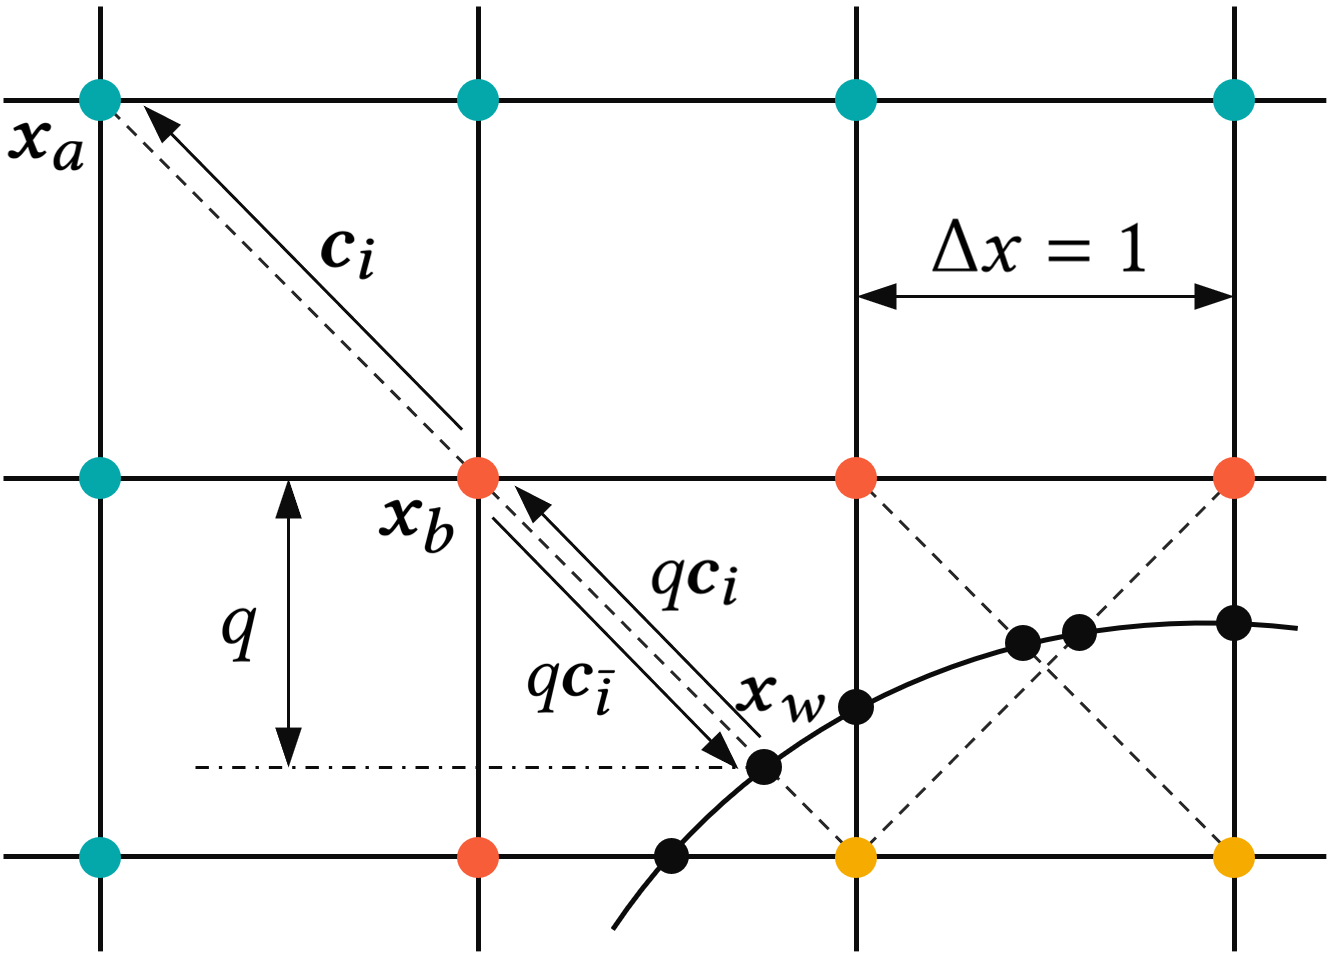
\includegraphics[width=0.7\columnwidth]{figures/boundary.png}
  \bicaption{固体附近的边界处理。对于切削网格点 (图中标为橘色),它们的未知分布函数必须要通过边界处理决定。图中黄色点为固体内部点,青色点为流体点。对于$\bm{x}_b$点,$q$表达该点沿$\bm{c}_i$方向到边界的正则化距离,其中$\bm{c}_{\bar{i}}$为$\bm{c}_i$的反方向。}{Boundary treatment near solid object. For ``cut-cell'' boundary nodes marked in orange, their unknown distribution functions must be determined through boundary schemes instead of the regular streaming. Yellow nodes mark nodes inside the solid while cyan nodes are fluids nodes. Our boundary treatment for a node $\bm{x}_b$ uses the normalized distance $q$ to the boundary surface along a link direction of $\bm{c}_i$ with its inverse direction denoted as $\bm{c}_{\bar{i}}$.}
  \label{img:boundary}
\end{figure}

\begin{figure}[htb]
	\centering
	  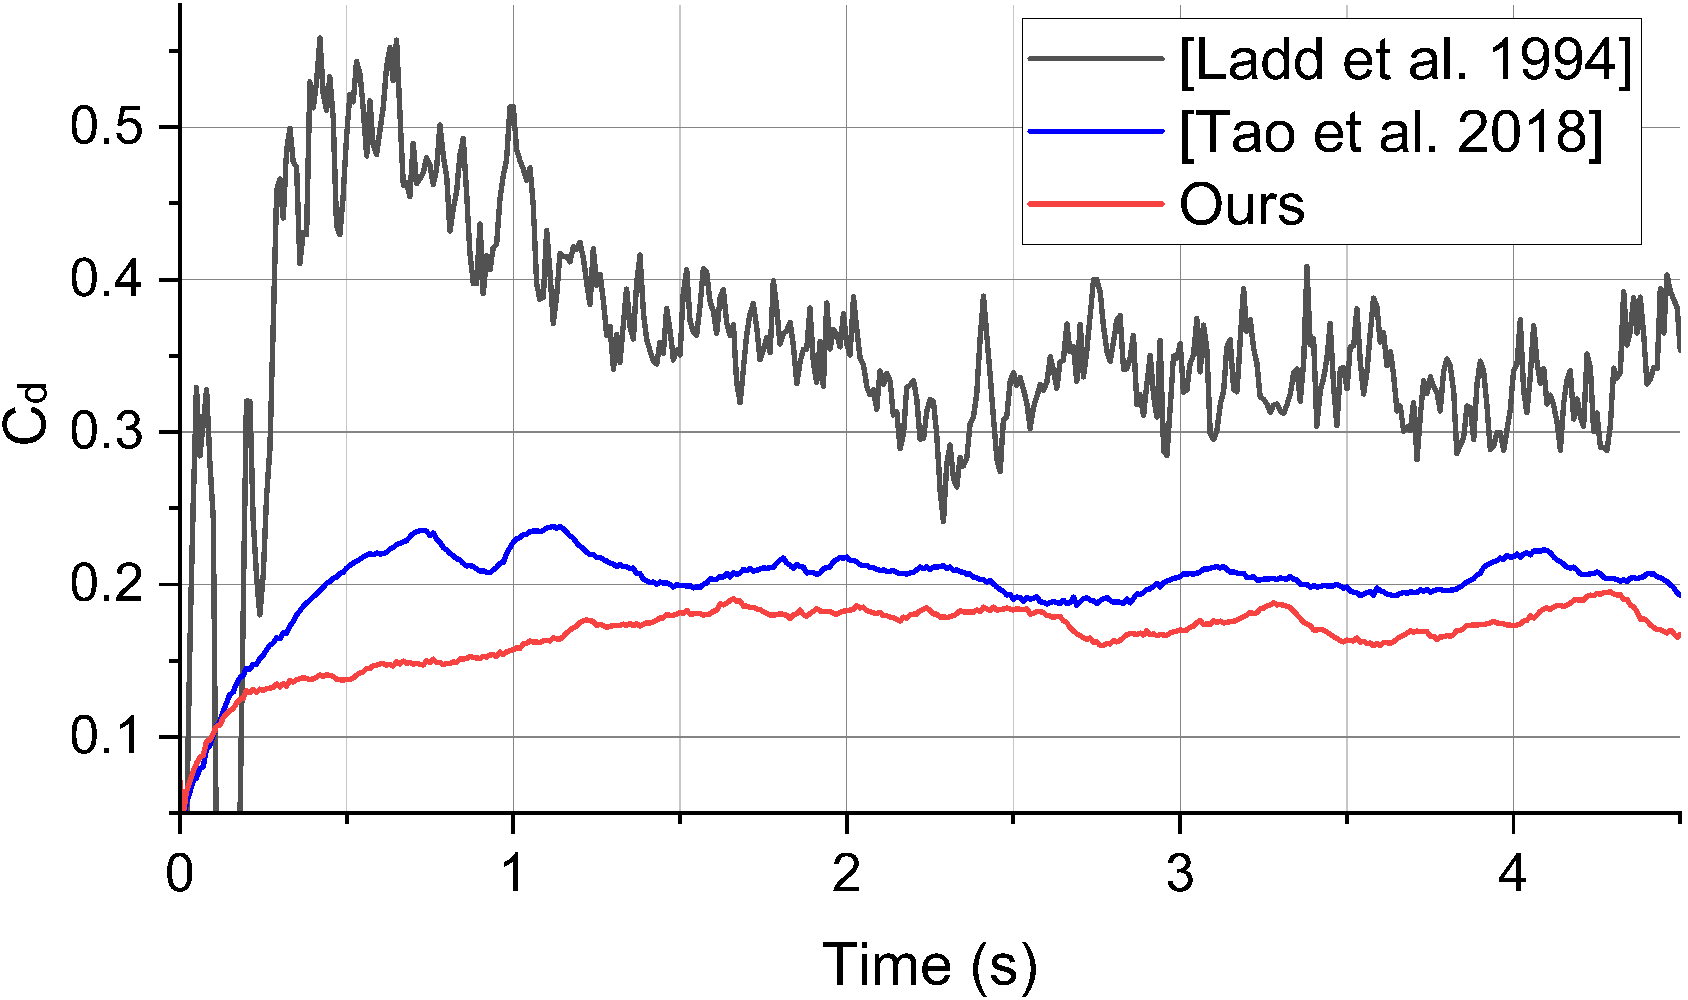
\includegraphics[width=0.8\columnwidth]{figures/bnd_comp.png}
	\bicaption{边界处理的比较。对于$Re=400,000$风吹过球的场景,我们画出了使用不同边界处理进行仿真得到的球的阻力系数。仿真中的碰撞模型均为使用了熵优化的累积量碰撞模型。该场景在实际实验中得到的球的阻力系数$C_\text{d}\!=\!0.1$。虽然简单反弹边界依然在许多LBM中得到应用,但是其结果误差及波动均过大,无法得到可置信的结果。}{Comparing boundary treatments. We plot the variation over time of drag coefficient of a sphere at $Re=400,000$, for different boundary treatments but with the same entropy-optimized cumulant model. The experimental value is near $C_\text{d}\!=\!0.1$ for this drag crisis case; a simple bounce-back, still used in many LBM implementations, leads to unacceptable results, producing large prediction errors and wide force fluctuations.}
	\label{img:bnd_comp}
  \end{figure}

在虚拟风洞中,在计算域中通常会有一个物体以进行气动性能测试,所以边界处理的重要性是不言而喻的。边界处理的示意图见图~\ref{img:boundary}。其中橘色点为需要进行边界处理的流体点,黄色点为固体内部点。
我们在第~\ref{sec:boundary_treatment} 节中已经讨论了简单反弹边界和插值反弹边界的形式。其中简单反弹边界虽然构造形式非常简单,但是在边界形状复杂时,一般只有一阶精度。从而在计算固体受力时,误差及波动是非常剧烈的 (见图~\ref{img:bnd_comp} 中展示的风在高雷诺数下吹过球时,球的阻力系数$C_\text{d}$变化)。
插值反弹边界~\cite{Bouzidi-2001} 与其之后的变体~\cite{Yu-2003, Ginzburg-2003, Chun-2007} 则可以使边界求解的精度达到二阶或更高。然而,这些边界处理方法均需要相邻点的参与,使得计算不再完全局部。由于GPU并行计算中,不连续数据访问对并行效率有很大影响,这样的边界处理在GPU计算上的效率有所降低。此外,当边界点周围均为边界时,找不到相邻点会使这样的边界处理方法失效。
而最近,Tao等~\citeyear{Tao-2018-b}) 通过在边界上构造额外的分布函数,提出了一个单点的插值反弹边界方法。
具体地,如图~\ref{img:bnd_comp}中所描绘的,我们用$\bm{x}_{b}$表达固体边界附近需要边界处理的点,$\bm{c}_{i}$为指向$\bm{x}_{a}$的方向,$\bm{c}_{\bar{i}}$为相反的方向并与固体边界相交于$\bm{x}_{w}$。跟随之前的方法中的假设,我们认为这之中存在线性关系:
\begin{equation}
f_i(\bm{x}_b, t\!+\!1) = \frac{1}{1+q}f_{i}(\bm{x}_w, t\!+\!1)+ \frac{q}{1+q}f_{i}(\bm{x}_a, t\!+\!1) \;,
\end{equation}
其中$q=\|\bm{x}_b - \bm{x}_w\|/\|\bm{c}_i\|$是边界点到边界的正则化距离。
然而分布函数$f_{i}(\bm{x}_a, t+1)$可以从$\bm{x}_b$的前一时刻迁移过来,所以这里的线性插值实际上只涉及一个点的数据。
此外,边界上的未知分布函数$f_{i}(\bm{x}_w, t\!+\!1)$可以由平衡态$f_{i}^\text{eq}(\bm{u}_w(t), \rho_b(t))$ ($\bm{u}_w(t)$为边界点的速度) 与非平衡态$f_{i}^\text{neq}(\bm{x}_b, t)$的和构造。$f_{i}^\text{neq}(\bm{x}_b, t)$可以表达为
\begin{equation}
f_{i}^\text{neq}(\bm{x}_b, t) = f_{i}(\bm{x}_b, t) - f_{i}^\text{eq}(\bm{u}_b, t),
\end{equation}
即将$\bm{x}_b$的非平衡态反转。
然而由于这样的构造使用了低阶的泰勒展开近似,在高雷诺数仿真中精度并不足够。为了进一步提升精度,我们提出一种新的构造平衡态和非平衡态的方法。
首先,我们利用非平衡态的阶数比平衡态高一阶的情况~\cite{Chun-2007},意味着我们可以对$\bm{x}_b$点的非平衡态进行简单反弹,获得的解依然是二阶精度。用公式表达为
\begin{equation}
\label{eq:neq_bb}
f^\text{neq}_{i}(\bm{x}_b, t\!+\!1) = f^\text{neq}_{\bar{i}}(\bm{x}_b, t).
\end{equation}
对于平衡态部分,我们可以采用与Tao等~\citeyear({Tao-2018-b}) 同样的二阶精度单点插值方法
\begin{align}
f^\text{eq}_i(\bm{x}_b, t\!+\!1) &= \frac{1}{1+q}f^\text{eq}_{i}(\bm{x}_w, t\!+\!1) + \frac{q}{1+q}f^\text{eq}_{i}(\bm{x}_a, t\!+\!1).
\end{align}
虽然$f^\text{eq}_{i}(\bm{x}_w, t\!+\!1)$可以由$f_{i}^\text{eq}(\bm{u}_w(t), \rho_b(t))$近似,但我们仍然需要确定如何求得$f^\text{eq}_{i}(\bm{x}_a, t\!+\!1)$。
由于我们无法获得$t+1$时刻的宏观量,一种方法是通过宏观量$\bm{u}(\bm{x}_a, t)$与$\rho(\bm{x}_a, t)$来重建平衡态。这样的做法相当于将平衡态公式对$t$进行泰勒展开后,进行了0阶逼近。这样的逼近势必在高雷诺数仿真中对边界层附近有负面的影响。
所以,我们利用$f^\text{eq}_{i}(\bm{x}_a, t\!+\!1) \approx f_{i}(\bm{x}_a, t\!+\!1)$来进行逼近,以不进行任何截断。并且$f_{i}(\bm{x}_a, t\!+\!1)$可以直接从$\bm{x}_b$迁移获得。所以我们得到
\begin{equation}
\label{eq:eq_a}
f^\text{eq}_{i}(\bm{x}_a, t\!+\!1) \approx f^{*}_{i}(\bm{x}_b, t).
\end{equation}
结合公式~\ref{eq:neq_bb}与公式~\ref{eq:eq_a},未知分布函数$f_i(\bm{x}_b, t\!+\!1)$可以被写为
\begin{align}
f_i(\bm{x}_b, t\!+\!1) &= f^\text{eq}_i(\bm{x}_b, t\!+\!1) + f^\text{neq}_{i}(\bm{x}_b, t\!+\!1) \\
&= \frac{1}{1\!+\!q}f_{i}^\text{eq}(\bm{u}_w(t), \rho_b(t)) + \frac{q}{1\!+\!q}f^{*}_{i}(\bm{x}_b, t) + f^\text{neq}_{\bar{\imath}}(\bm{x}_b, t).\nonumber
\end{align}

\paragraph{动态耦合}
虚拟风洞中也需要一部分动态的单向耦合,如汽车上轮胎的旋转。
之前的LBM通常结合格点重填与反弹边界条件~\cite{Tao-2016},或使用浸没边界法~\cite{Li-2016, Li-2020}进行动态耦合。
格点重填结合反弹边界条件的方法在高雷诺数仿真中会在边界周围产生不正常的速度,而浸没边界法虽然更容易实现,但因为只有一阶精度,则达到同样精度需要更高的分辨率进行仿真,从而消耗更多的资源。
为了保证在薄边界层上保证更高的精度,在动态耦合时,我们依赖于上述的静态边界处理方法,不同点是现在各个切削速度方向的$\bm{u}_w$都需要求解。并且我们依然使用\emph{浸没}的模式来处理边界,以避免格点重填。即所有的格点我们都认为是流体点,没有固体点。当然我们注意到,要在每个时间步都进行求交并求解边界的速度,通常需要进行层级搜索~\cite{Karras-2012},而当分辨率非常高时,在GPU上进行这样的操作非常耗时。
于是我们提出了相应的GPU实现,以减轻求交与动态耦合的计算开销。这些算法我们在第 \TODO{XXX} 章中介绍。

\paragraph{固体受力计算}
对于上述的边界处理,我们依然可以用动量交换法计算固体受力~\cite{Ladd-1994, Mei-2002},即对于边界点$\bm{x}$有
\begin{equation}
    \Delta \bm{p}(\bm{x})= \sum_{j\in L(\bm{x})} \bm{c}_{j'}\,(f_{j}(\bm{x}) + f^*_{j'}(\bm{x})),\vspace*{-1.5mm}
\end{equation}
其中$L(\bm{x})$为$\bm{x}$点向外的速度方向 (由固体向流体方向),$f_{j}(\bm{x})$为通过边界处理方法得到的分布函数。则固体受到的合力为所有边界点上受力的和
\begin{equation}
    \bm{F} = \sum_{\bm{x}} \Delta \bm{p}(\bm{x}).\vspace*{-1mm}
\end{equation}
注意因为我们使用了浸没的思想,所以所有的切削网格点都应被视为边界点。

% \subsection{Multiresolution simulation}
% \label{sec:multi-res}
% Running the simulation framework we described up to now on a single LBM grid would be enough for most CG applications looking to efficiently capture a fluid flow over relatively simple geometric models for visual purposes. But in an engineering context, a virtual wind tunnel must accommodate large domains (typically of size 40m$\times$20m$\times$20m for a 16-foot car model) with a constraint on resolving geometric details as small as 3mm typically to capture small-scale flow features well enough to ensure an accurate evaluation of key physical quantities. A single grid would thus have to be impractically large to fit these requirements, creating an unacceptable wall-clock time and memory storage for simulation. 
% Multiresolution simulation is thus an indispensable ingredient of a physically-accurate fluid simulator for engineering design, and grid refinement has thus been systematically adopted in most industrial simulators~\cite{Hou-2019,Aultman-2022,Romani-2022}.
% However, as argued before, many traditional FVM-based NS solvers usually require body-fitted unstructured meshes, for which a versatile and fully automatic mesh construction algorithm is extremely challenging to generate due to the complex geometry (and sometimes, topology) of the prototypes.
% In the LBM literature, multiresolution methods often employ octree-based grid data structure~\cite{EitelAmor-2013,Hasert-2014}, but their GPU implementations are quite involved~\cite{Schornbaum-2016, Schornbaum-2018}.
% Instead, we propose a fully automatic block-based multiresolution grid construction method for our LBM fluid simulator that is better adapted to efficient GPU implementation and can handle flows through extremely complex structures as described next.

% \paragraph{Multiresolution grid construction}
% Grid refinement is often guided by different criteria, among which incoming flow direction and distance to a model~\cite{Sandoval-2012,Li-2019} are arguably the most common choices.
% We thus designed our automatic multiresolution grid construction algorithm around these two factors.
% Given an axis-aligned bounding box (AABB) of the model, we first extend it by a certain distance $d^*$ representing the boundary layer thickness determined by the Reynolds number, in order to form a larger box-shaped region labeled $\Omega_n$ --- see the red box in Fig.~\ref{fig:grid_construction}.
% From the whole simulation domain $\Omega$, we then define the pure flow region $\Omega_f \!=\! \Omega \setminus \Omega_n$.
% Inside $\Omega_f$, we construct our multiresolution data structure based solely on the direction of the incoming flow by using axis-aligned grids of power-of-two resolutions which partially overlap (to ease grid transition); i.e., we go from coarse at the domain boundary to finest at $\Omega_n$ by ensuring that each uniform grid level is twice as fine as its parent while being offset from the center $\Omega_n$ along the incoming flow direction so as to cover more of the wake flow (where the turbulence must be well resolved) than in the front --- see how the regions from blue to yellow unevenly straddle the building in Fig.~\ref{fig:grid_construction}.
% As for inside $\Omega_n$, we refine the sampling once further compared to the finest grid level in $\Omega_f$, but this time we transition to a refinement based on the distance to the model: using an unsigned distance field of the model computed within $\Omega_n$, we use a once-refined uniform grid compared to the finest grid level in $\Omega_f$, and consider its nodes to be \emph{valid} only if they are within a distance $d^*$ of the model --- see the orange nodes in Fig.~\ref{fig:grid_construction}. Note that we use a mask per grid node to indicate whether or not it is a valid fluid node, and we adopt the efficient GPU-based approach of~\cite{Imre-2017} to compute the distance field. 
% The resulting multiresolution sampling is thus block-based and independent, as it does not form a tree-like hierarchy --- but it allows for a good transition between multiple levels of resolutions without the prohibitive memory storage required by the continuous-scale approach of \cite{Li-2019}, for instance.

% \paragraph{Dynamic objects}
% Because of the specific nature of a wind tunnel facility, we can restrict our handling of dynamic objects in a simulation with one-way coupling to mostly rotations, such as the wheels of a car spinning. From an axis-aligned bounding box of the rotating object, 
% we construct a grid with the finest resolution and set all its nodes as valid fluid nodes. More complex motions, such as the opening of a plane's wheel well with the landing gear coming out, can in fact be handled the same way, but one must then pick an axis-aligned bounding box that encloses the complete motion of the dynamic objects, which can be potentially wasteful in the number of finest nodes depending on the scenario at hand. We leave such very specific improvements to future work.

% \begin{figure}[t] %\vspace*{0mm}
% 	\centering 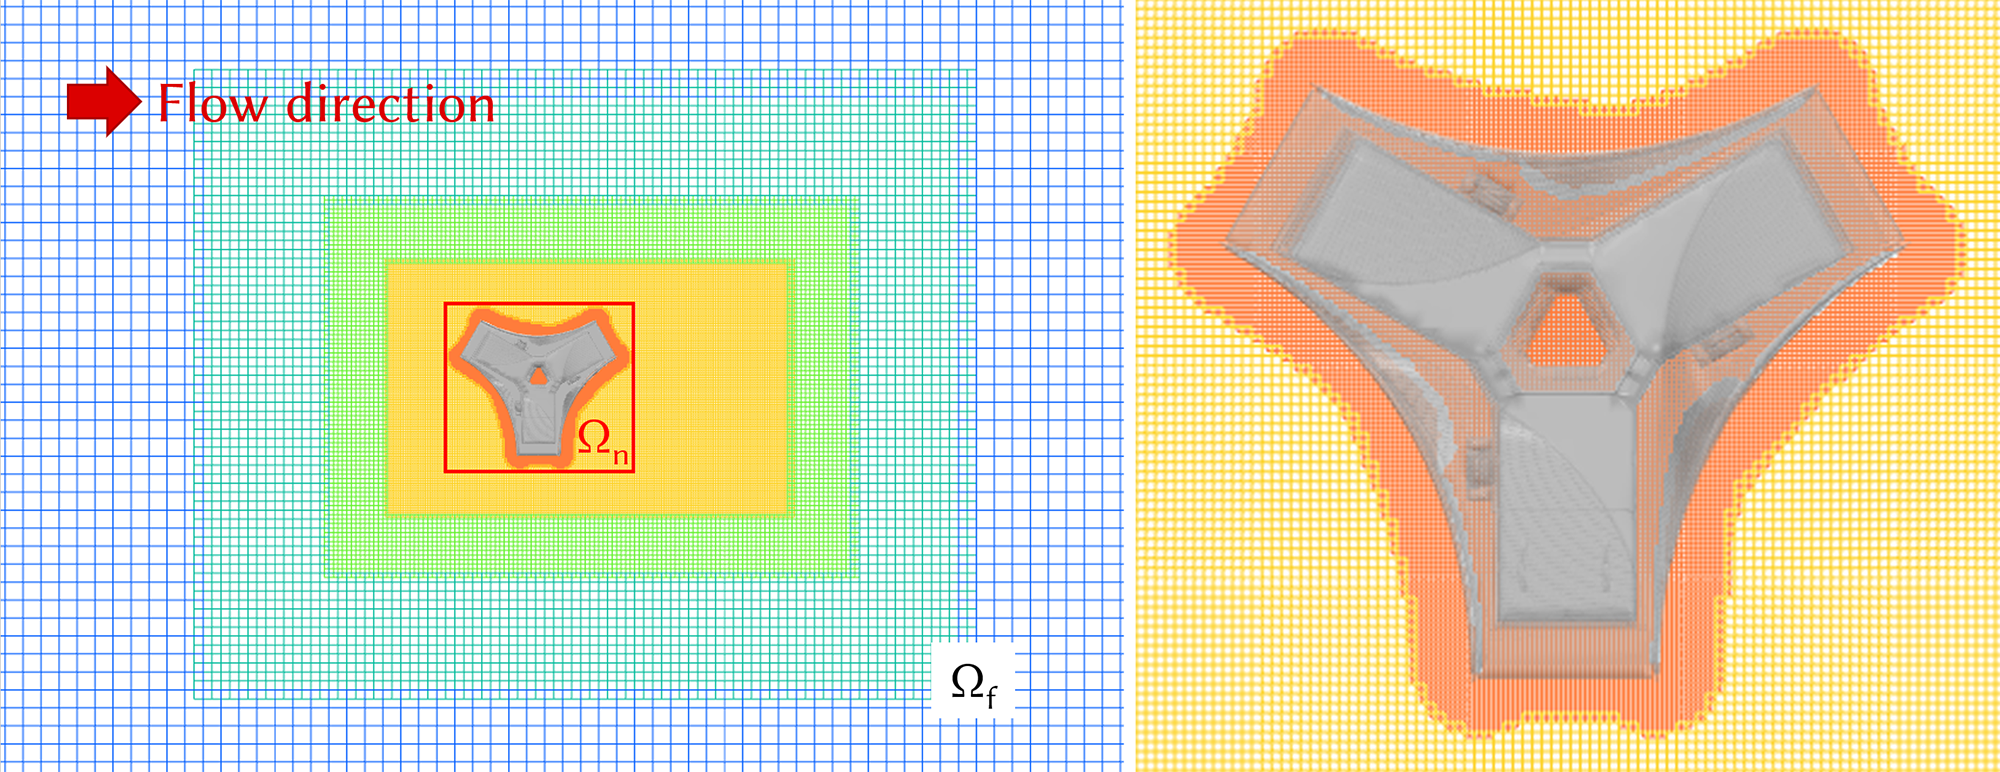
\includegraphics[width=0.9\columnwidth]{images/grid_construction}\vspace*{-2.5mm} 
% 	\caption{\textbf{Multiresolution grid construction.} To keep memory size low when computing accurate predictions of physical quantities, multiresolution grids are automatically constructed, with a refinement guided by the incoming flow direction for all but the last grid level (left) --- explaining the offset of the different levels of grid compared to this architectural building so as to capture its wake accurately --- then by the distance to the object. All active fluid nodes are finally found by flooding to ensure that the flow goes through all the mesh openings larger than the finest grid resolution (right).\vspace*{-3mm} }
% 	\label{fig:grid_construction}
% \end{figure}

% \paragraph{Dealing with complex models}
% %Propagation of valid fluid nodes}
% We assumed until now that the model surface is closed, for which using a signed distance is sufficient to identify valid fluid regions.
% However, in real applications, many models are not truly closed: e.g., a car may have a grill wire as an external air inlet, or an architectural model can have small openings, still larger in size than the finest grid cell, to let the wind flow inside parts of the building.
% In this case, the above grid construction is not sufficient: we
% must run a flooding algorithm on the \emph{finest} grid level to properly tag as valid the nodes that are connected to the external flow. 
% Starting from a known fluid node ---  e.g., the node at the corner of the region $\Omega_n$ --- we check its 6 neighbor nodes and perform link-surface intersection to see whether a neighboring node is connected to the current fluid node, see Fig.~\ref{fig:propagation} in 2D as an illustration. 
% Only if a neighboring node is connected to the current fluid node do we mark it as a valid fluid node, and we propagate through the valid fluid nodes using a breath-first search order such that all fluid nodes inside $\Omega_n$ are visited.

% %Fig.~\ref{fig:grid_construction} shows the multi-resolution grid construction the right figure shows the fluid grids constructed automatically inside the geometry where the domain is connected to the exterior. 
% %m@: pointless, no? the figure does not show which one is valid, which was is not.

% \paragraph{Grid interpolation}
% Our multiresolution grid construction enforces that only \emph{two} grids that are one level apart can overlap.
% We must therefore define how to evaluate and update in time the distribution functions at a given node based on the values stored on these two levels.
% For this purpose, we strictly follow the approach described in~\cite{Lagrava-2012}. 
% The internal nodes of a coarser parent grid provide boundary values which allow the finer grid to be updated twice (since a twice-finer grid requires twice-smaller integration time steps in LBM), where the distribution functions at the boundary nodes of the finer grid are readily interpolated from the coarser grid at the current time step.
% Then, the boundary nodes of the coarser grid can be updated by interpolating from the already updated finer grid at the next time step, and so on. 
% The interpolation is done by separating the distribution functions into equilibrium and non-equilibrium parts, where the equilibrium part is computed by first interpolating macroscopic quantities before evaluating its equilibrium distribution values, while the non-equilibrium part is interpolated directly; both interpolations are done using high-order schemes~\cite{Lagrava-2012}. 
% This process is applied recursively from the coarsest grid to the finest grid in a cascaded serialized manner.
% Fig.~\ref{fig:vis_building} for instance shows an instantaneous macroscopic velocity field cross-section from the simulation of the same architecture model from Fig.~\ref{fig:grid_construction} using this interpolation approach.

% \begin{figure}[t] %\vspace*{0mm}
% 	\centering 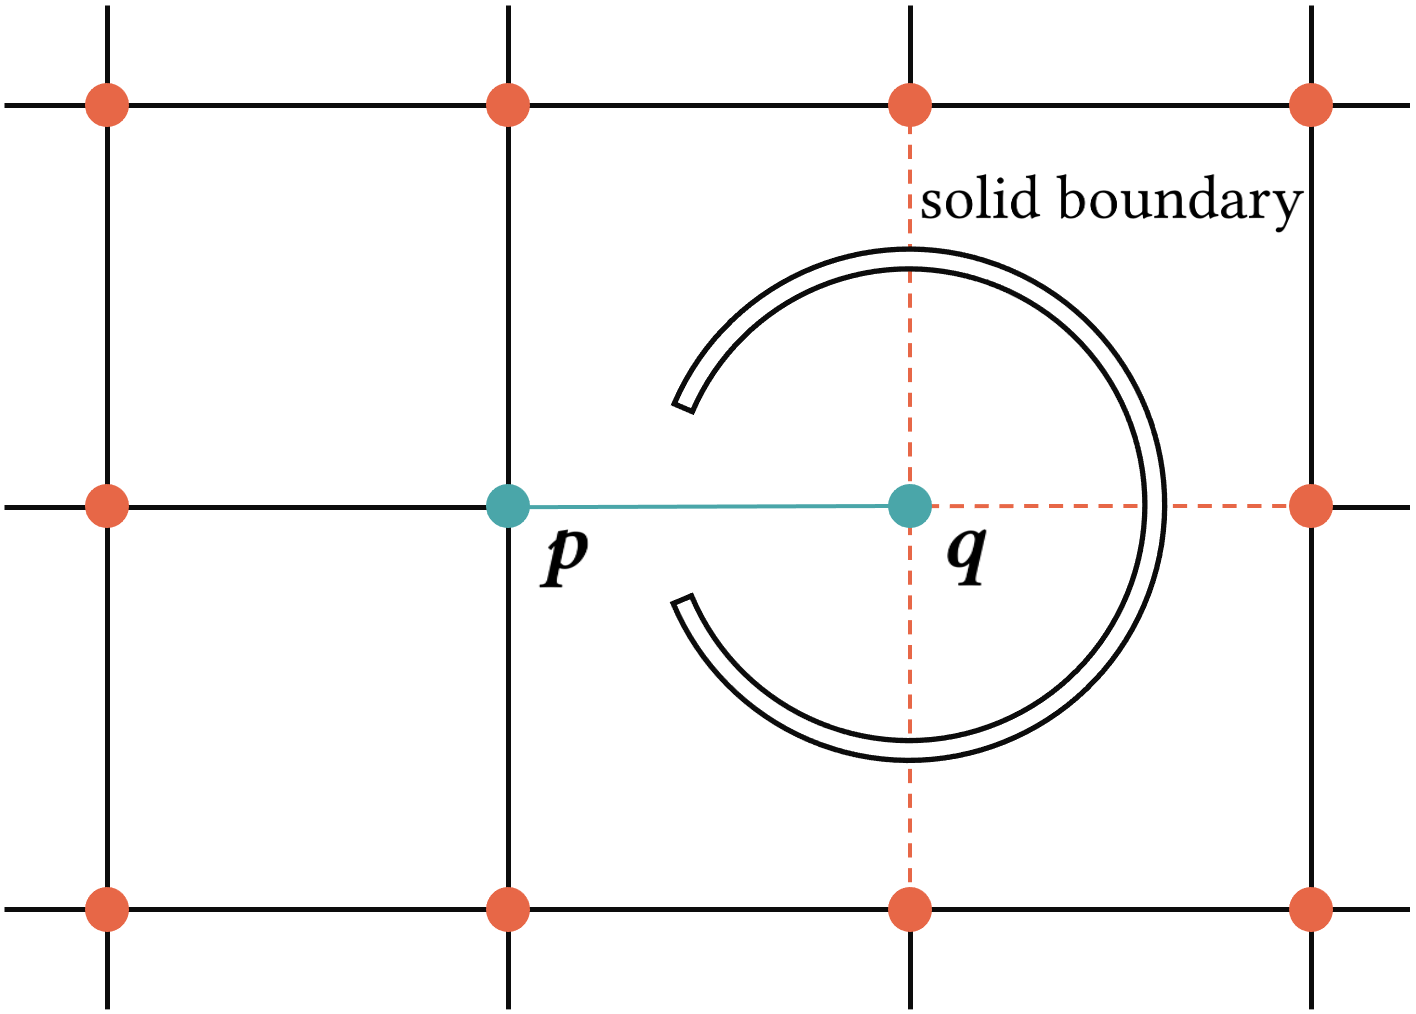
\includegraphics[width=0.55\columnwidth]{images/propagation}\vspace*{-3mm} 
% 	\caption{\textbf{Propagation of valid fluid nodes.} To find and tag all valid fluid nodes, we start from an already known fluid node, e.g., node $\bm{p}$ in 2D, then we check its immediate neighbors to see whether a link intersects a boundary. If no intersection is detected (e.g., link $\bm{p}\bm{q}$), the untagged node $\bm{q}$ is tagged as a new valid fluid node. This process repeats in a bread-first search order, enabling internal regions to be connected to the external fluid region.  \vspace*{-3mm}}
% 	\label{fig:propagation}
% \end{figure}